\subsection{Sprachenmodell}
\label{sec:language_model}

Die Aufgabe des Generators ist die Transformierung des Applikationsmodells in das Modell der Zielsprache. 

Um die gewünschte Austauschbarkeit der Zielsprache zu gewährleisten wurde ein abstraktes Sprachenmodell entworfen welches die Konstrukte einer dateibasierten Objektorientierten Programmiersprache (siehe \cref{sec:oo_languages}) abbildet. 
%Anforderungen erstellen und referenzieren.
Die gewünschte Zielsprache muss dabei die Klassen und Methoden des Modells implementieren sowie eine \emph{Language Factory} (siehe \cref{sec:language_factory}) bereitstellen um vom Generator genutzt werden zu können.
Abgesehen von Symbolen und Schlüsselwörtern wird die Syntax der Zielsprache in der Klasse \emph{LanguageVisitor} (siehe \cref{sec:language_visitor}) gekapselt. 

Alle Interfaces des Modells (siehe \cref{fig:language_model}) erweitern das Interface \textbf{Visitor}, somit ist sichergestellt das alle Klassen die diese Schnittstellen implementieren eine \emph{accept}-Methode für den \emph{LanguageVisitor} bereitstellen.

Basis des Modells ist das Interface \textbf{ClassFile}, es abstrahiert eine Klassendatei mit den Eigenschaften:
\begin{compactitem}
    \item Dateiname
    \item Namensraum
    \item Liste von Abhängigkeiten (\emph{Dependency}-Klasse)
    \item Klassendefinition
\end{compactitem}

Die Liste von Abhängigkeiten der zu generierenden Klassen muss vorher aus dem Eingabemodell ermittelt werden, dies geschieht durch Analyse der in den Elementdefinitionen des Schemamodells enthaltenen Typen. 

\textbf{Dependency} enthält das Schlüsselwort oder Methodenaufruf zum Import einer Quellcodedatei. In PHP werden solche Dateien bpsw. so importiert: \texttt{require\_once("foo.php");}.

\textbf{Executable} implementieren alle Elemente der Zielsprache die \enquote{ausführbar} sind. Das Modell unterscheidet dabei zwischen \emph{Ausdruck} und \emph{Anweisung} (siehe \cref{sec:oo_languages}). 
Das Interface \textbf{CommonClass} dient zur Implementierung einer Klassendefinition. Da das Interface selbst \emph{Statement} erweitert, kann eine Klasse weitere Klassendefinitionen beinhalten. Eine Klassendefinition besteht dabei aus einem Klassename, Modifiers und aus einer Menge von Statements:
\begin{compactitem}
    \item \emph{DefinitionStatement} zur Einführung von lokalen Variablen.
    \item \emph{Method} zur Definition von Methoden.
\end{compactitem}

Das \textbf{Modifier}-Interface beschreibt Methoden um die Schlüsselwörter für Sichtbarkeitsmodifikatoren (\enquote{Access Modifier}) und \enquote{Non Access Modifiers} wie \texttt{static} oder \texttt{final}, zu erhalten.

Durch das \textbf{Method}-Interface kann eine Methodendefinition implementiert werden. Eine Methode beinhaltet dabei:
\begin{compactitem}
    \item Modifier
    \item Methodenname
    \item Rückgabetyp
    \item Liste von Parametern % todo: liste von variablen, wie abstrahiert?
    \item \emph{Block}
\end{compactitem}

\textbf{Block} kapselt eine Menge von Statements.

Operatoren der Zielsprache müssen das Interface \textbf{Operator} implementieren, ein Operator ist durch seine Arität (Stelligkeit), Notation und sein Symbol gekennzeichnet. Zum Beispiel der Dereferenzierungsoperator in PHP ist zweistellig, Infix notiert und wird gekennzeichnet durch das Symbol \texttt{->}.

\textbf{Keywords} und \textbf{Symbols} dienen zur Kapselung der Schlüsselwörter und Symbole einer Sprache. Keywords enthält Methoden zur Abfrage typischer Schlüsselworte wie \emph{class}, \emph{import}, \emph{new} oder \emph{this}. Sprachspezifische Symbole wie \emph{Verkettungs}- und \emph{Scope}-Operatoren oder Präfixe für Variablennamen können über Methoden der Klasse Symbols vom Generator abgefragt werden.

\begin{sidewaysfigure}
    \centering
    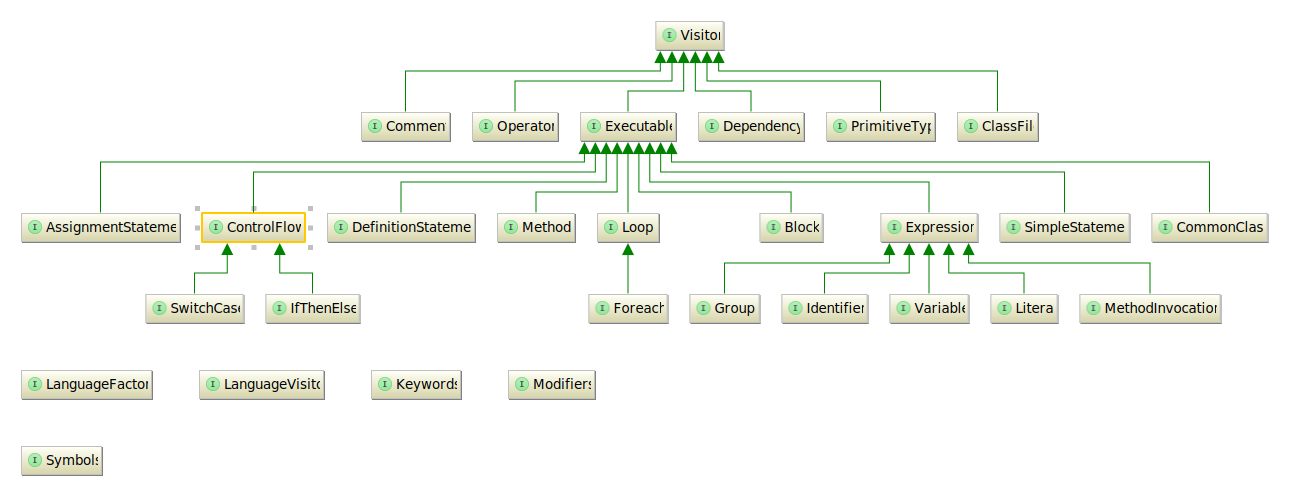
\includegraphics[width=\textheight]{resources/languagemodel_common}
    \caption{UML Klassendiagramm des Zielsprachenmodells}
    \label{fig:language_model}
\end{sidewaysfigure}
